\documentclass[11pt,slovak,a4paper,usepdftitle=false]{article}

\usepackage[slovak]{babel}
\usepackage[T1]{fontenc}
\usepackage[utf8]{inputenc}
\usepackage{graphicx}
\usepackage{url} % \url
\usepackage{hyperref} % Automatic links
\usepackage{parskip}
\usepackage[left=2cm, right=2cm]{geometry}
\usepackage{listings}
\usepackage{xcolor}
\usepackage{amsmath}
\usepackage{placeins}
\usepackage{cite}
\usepackage{listings}
\usepackage{xcolor}
\usepackage{pgfkeys}
\usepackage{pdfpages}
\usepackage{tabto}
\usepackage{enumitem}
\usepackage{longtable}

\newcommand{\spc}{\,}

\setlist{itemsep=0.4em, parsep=0em, midpenalty=3000}

\hypersetup{pdftitle=Generátor plošinových hier,pdfdisplaydoctitle}

\pgfkeys{
    /codeblock/.is family, /codeblock,
    default/.style = {start = 1, end = 1, language=None},
    start/.estore in = \codeblockStart,
    end/.estore in = \codeblockEnd,
    language/.estore in = \codeblockLanguage,
}
\newcommand\codeblock[2][]{\pgfkeys{/codeblock, default, #1}\lstinputlisting[firstnumber=\codeblockStart,firstline=\codeblockStart,lastline=\codeblockEnd,language=\codeblockLanguage]{#2}}

\definecolor{codegreen}{rgb}{0,0.6,0}
\definecolor{codegray}{rgb}{0.5,0.5,0.5}
\definecolor{codedark}{rgb}{0.3,0.3,0.3}
\definecolor{codepurple}{rgb}{0.58,0,0.82}

\lstdefinestyle{mystyle}{ 
    commentstyle=\sffamily\color{codegreen},
    keywordstyle=\color{magenta},
    numberstyle=\tiny\color{codegray},
    stringstyle=\color{codepurple},
    basicstyle=\ttfamily\footnotesize\color{codedark},
    breakatwhitespace=true,
    identifierstyle=\color{black},      
    breaklines=true,                 
    captionpos=b,                    
    keepspaces=true,                 
    numbers=left,                    
    numbersep=5pt,                  
    showspaces=false,                
    showstringspaces=false,
    showtabs=false,                  
    tabsize=4
}

\lstdefinelanguage{json}
{
    morestring=[b]",
    morestring=[d]'
}

\lstset{
	style=mystyle,
	inputencoding=utf8,
    columns=fullflexible,
	literate={ú}{{\'u}}1 {í}{{\'i}}1 {á}{{\'a}}1 {ĺ}{{\'l}}1 {é}{{\'e}}1 {ý}{{\'y}}1 {ó}{{\'o}}1 {ž}{{\v{z}}}1 {š}{{\v{s}}}1 {ď}{{\v{d}}}1 {č}{{\v{c}}}1 {ň}{{\v{n}}}1 {ť}{{\v{t}}}1 {ľ}{{\v{l}}}1 {ä}{{\"{a}}}1 {Δ}{{\ensuremath{\Delta}}}1
}

\DeclareUnicodeCharacter{21D2}{\ensuremath{\Rightarrow}}

\renewcommand{\familydefault}{\sfdefault} % Sans serif
\raggedright

% použiť hiearchiálne ordered lists
\renewcommand{\labelenumii}{\theenumii}
\renewcommand{\theenumii}{\theenumi.\arabic{enumii}.}

\renewcommand{\labelenumiii}{\theenumiii}
\renewcommand{\theenumiii}{\theenumii\arabic{enumiii}.}

\renewcommand{\labelenumiv}{\theenumiv}
\renewcommand{\theenumiv}{\theenumiii\arabic{enumiv}.}

\pagestyle{plain}
\pagenumbering{roman}

\begin{document}


\includepdf[pages=-]{ref-title-page.pdf}

% zadná strana titulného listu (prázdna strana)
\null \thispagestyle{empty}

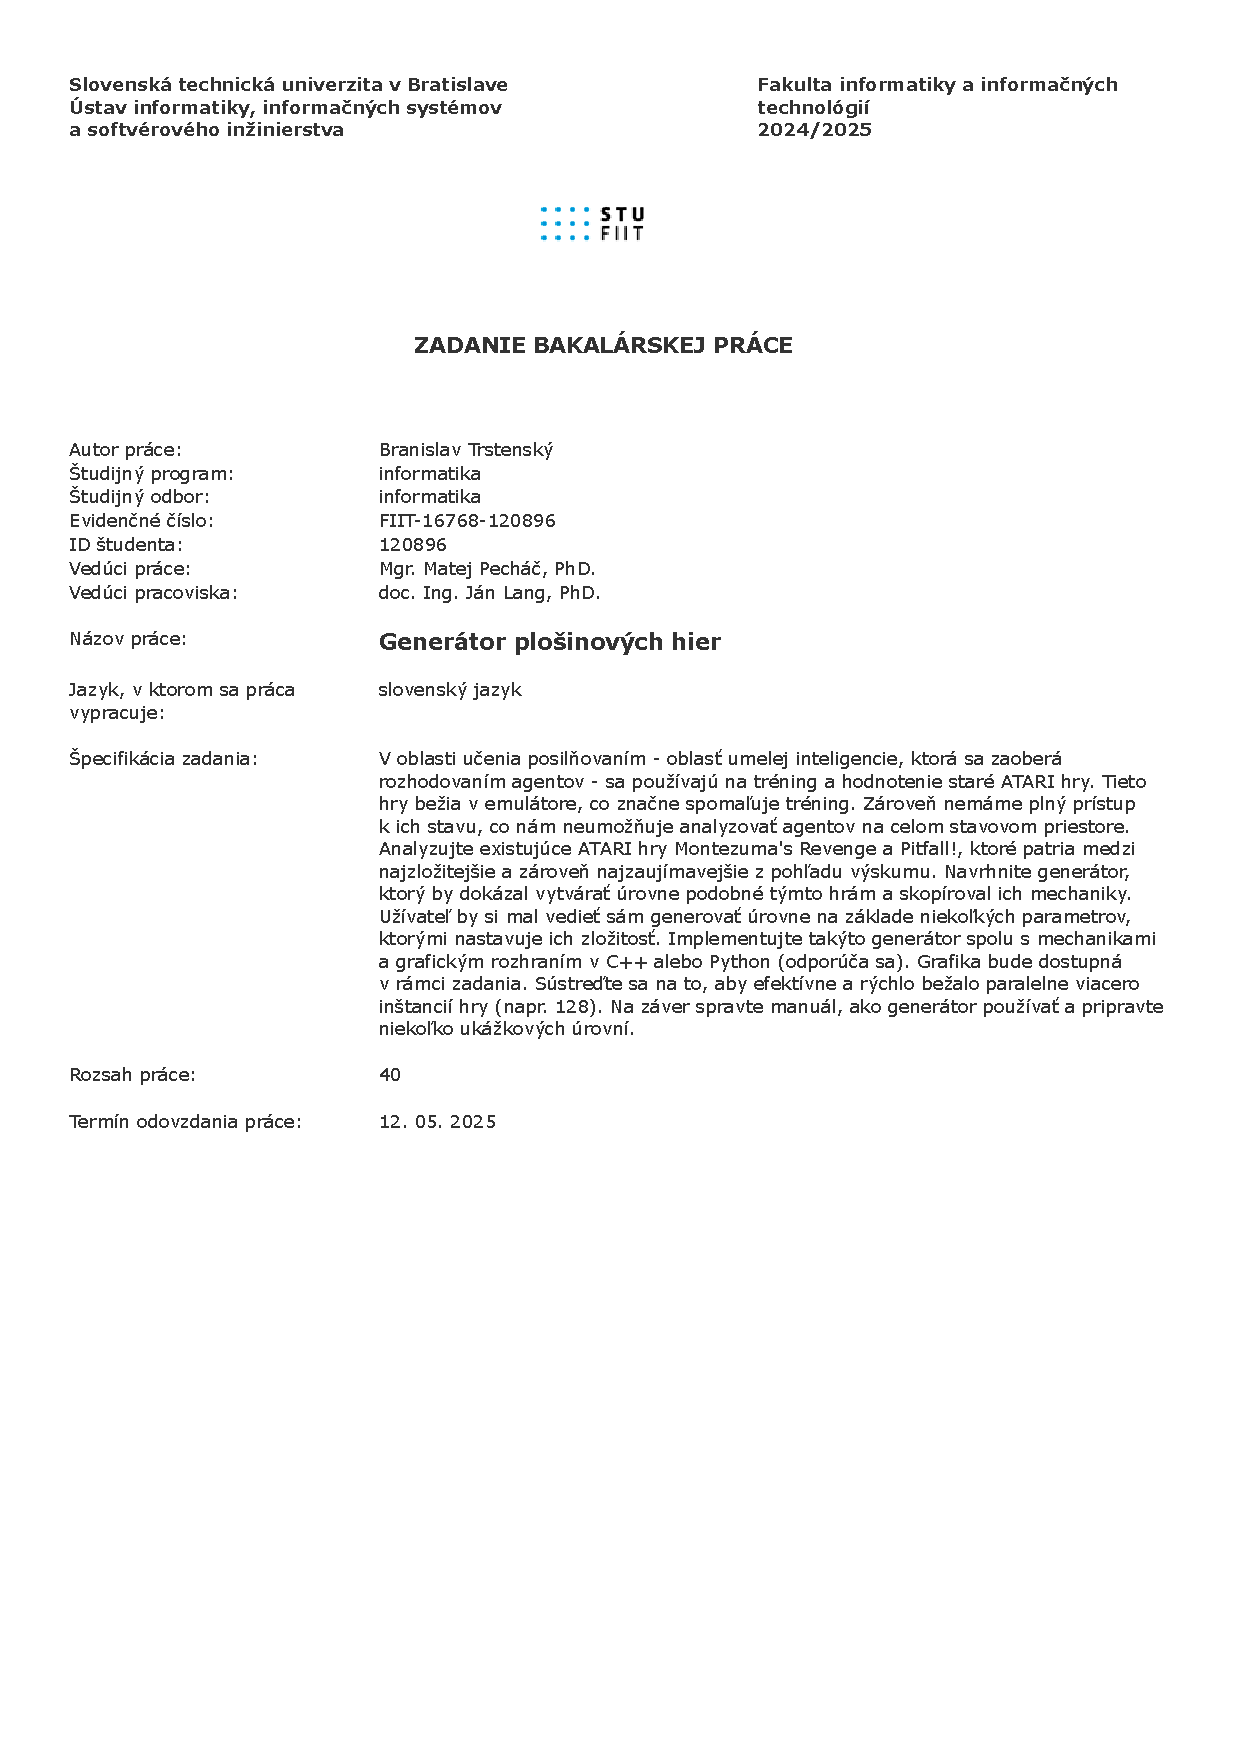
\includepdf[pages=-]{ref-zadanie.pdf}

% zadná strana zadania/revízie (môže byť prázdna)
\null \thispagestyle{empty}

\newpage

% čestné vyhlásenie je napísané na spodku strany
\null \thispagestyle{empty} \vfill

Čestne vyhlasujem, že som túto prácu vypracoval(a) samostatne, na základe konzultácií
a s použitím uvedenej literatúry.

V Bratislave, \today.

\begin{flushright}
    Branislav Trstenský
\end{flushright}

\newpage

% zadná strana čestného prehlásenia (prázdna strana)
\null \thispagestyle{empty}

\newpage

\section*{Anotácia}

Slovenská technická univerzita v Bratislave

FAKULTA INFORMATIKY A INFORMAČNÝCH TECHNOLÓGIÍ

\NumTabs{3}

Študijný program: \tab informatika

Autor: \tab Branislav Trstenský

Bakalárska práca: \tab Generátor plošinových hier

Vedúci diplomovej práce: \tab Mgr. Matej Pecháč, PhD.

Január 2025


Pri spätnoväzobovom učení, v oblasti umelej inteligencie zaoberajúcej sa rozhodovaním agentov, sa používajú na tréning a hodnotenie staré ATARI hry. Tieto hry bežia v emulátore, čo značne spomaľuje tréning. Zároveň nemáme plný prístup k ich stavu, čo nám neumožnuje analyzovať agentov na celom stavovom priestore. 

Táto práca sa zaoberá vytvorením generátora, ktorý je schopný vytvoriť úrovne podobné ATARI hrám,  ako sú Pitfall! alebo Montezuma's Revenge, ktoré patria medzi najzložitejšie a zároveň najzaujímavejšie z pohľadu výskumu.

Generátor umožňuje používateľovi jednoducho vytvoriť nové úrovne nastavením malého počtu parametrov. Tiež je jeho súčasťou replikácia mechaník týchto hier, čo umožňuje tieto hry spustiť pre použitie s agentom umelej inteligencie.

\newpage

% zadná strana anotácie (prázdna strana)
\null \thispagestyle{empty}

\newpage

\section*{Annotation}

Slovak University of Technology Bratislava

FACULTY OF INFORMATICS AND INFORMATION TECHNOLOGIES

\NumTabs{3}

Degree course: \tab informatika

Autor: \tab Branislav Trstenský

Bachelor's Thesis: \tab Platform game generator

Supervisor: \tab Mgr. Matej Pecháč, PhD.

Január 2025

For reinforcement learning, in the field of artificial intelligence dealing with agent decision-making, old ATARI games are used for training and evaluation. These games run in an emulator, which significantly slows down training. At the same time, we do not have full access to their state, which does not allow us to analyze agents in the entire state space.

This thesis deals with the creation of a generator capable of generating levels similar to ATARI games such as Pitfall! or Montezuma's Revenge, which are among the most complex and at the same time most interesting from a research point of view.

The generator allows users to easily create new levels by setting a small number of parameters. It also includes a replica of the mechanics of these games, which allows these games to be run for use with an artificial intelligence agent.

\newpage

% zadná strana anotácie (prázdna strana)
\null \thispagestyle{empty}

\newpage

\thispagestyle{plain}
\tableofcontents

\newpage

% posledná zadná strana obsahu (alebo zoznamov) (ak je prázdna, číslo strany sa neuvádza)
\null \thispagestyle{empty}

\newpage

\setcounter{page}{1}
\pagenumbering{arabic}

\widowpenalties 1 10000
\input{doc.tex}

\newpage

\Urlmuskip=0mu plus 1mu
\def\UrlBreaks{\do\/\do-}

\addcontentsline{toc}{section}{Literatúra}
\bibliography{bibliography}
\bibliographystyle{stn690}


\end{document}
